\documentclass[twoside]{book}

% Packages required by doxygen
\usepackage{fixltx2e}
\usepackage{calc}
\usepackage{doxygen}
\usepackage[export]{adjustbox} % also loads graphicx
\usepackage{graphicx}
\usepackage[utf8]{inputenc}
\usepackage{makeidx}
\usepackage{multicol}
\usepackage{multirow}
\PassOptionsToPackage{warn}{textcomp}
\usepackage{textcomp}
\usepackage[nointegrals]{wasysym}
\usepackage[table]{xcolor}

% Font selection
\usepackage[T1]{fontenc}
\usepackage[scaled=.90]{helvet}
\usepackage{courier}
\usepackage{amssymb}
\usepackage{sectsty}
\renewcommand{\familydefault}{\sfdefault}
\allsectionsfont{%
  \fontseries{bc}\selectfont%
  \color{darkgray}%
}
\renewcommand{\DoxyLabelFont}{%
  \fontseries{bc}\selectfont%
  \color{darkgray}%
}
\newcommand{\+}{\discretionary{\mbox{\scriptsize$\hookleftarrow$}}{}{}}

% Page & text layout
\usepackage{geometry}
\geometry{%
  a4paper,%
  top=2.5cm,%
  bottom=2.5cm,%
  left=2.5cm,%
  right=2.5cm%
}
\tolerance=750
\hfuzz=15pt
\hbadness=750
\setlength{\emergencystretch}{15pt}
\setlength{\parindent}{0cm}
\setlength{\parskip}{3ex plus 2ex minus 2ex}
\makeatletter
\renewcommand{\paragraph}{%
  \@startsection{paragraph}{4}{0ex}{-1.0ex}{1.0ex}{%
    \normalfont\normalsize\bfseries\SS@parafont%
  }%
}
\renewcommand{\subparagraph}{%
  \@startsection{subparagraph}{5}{0ex}{-1.0ex}{1.0ex}{%
    \normalfont\normalsize\bfseries\SS@subparafont%
  }%
}
\makeatother

% Headers & footers
\usepackage{fancyhdr}
\pagestyle{fancyplain}
\fancyhead[LE]{\fancyplain{}{\bfseries\thepage}}
\fancyhead[CE]{\fancyplain{}{}}
\fancyhead[RE]{\fancyplain{}{\bfseries\leftmark}}
\fancyhead[LO]{\fancyplain{}{\bfseries\rightmark}}
\fancyhead[CO]{\fancyplain{}{}}
\fancyhead[RO]{\fancyplain{}{\bfseries\thepage}}
\fancyfoot[LE]{\fancyplain{}{}}
\fancyfoot[CE]{\fancyplain{}{}}
\fancyfoot[RE]{\fancyplain{}{\bfseries\scriptsize Generated by Doxygen }}
\fancyfoot[LO]{\fancyplain{}{\bfseries\scriptsize Generated by Doxygen }}
\fancyfoot[CO]{\fancyplain{}{}}
\fancyfoot[RO]{\fancyplain{}{}}
\renewcommand{\footrulewidth}{0.4pt}
\renewcommand{\chaptermark}[1]{%
  \markboth{#1}{}%
}
\renewcommand{\sectionmark}[1]{%
  \markright{\thesection\ #1}%
}

% Indices & bibliography
\usepackage{natbib}
\usepackage[titles]{tocloft}
\setcounter{tocdepth}{3}
\setcounter{secnumdepth}{5}
\makeindex

% Hyperlinks (required, but should be loaded last)
\usepackage{ifpdf}
\ifpdf
  \usepackage[pdftex,pagebackref=true]{hyperref}
\else
  \usepackage[ps2pdf,pagebackref=true]{hyperref}
\fi
\hypersetup{%
  colorlinks=true,%
  linkcolor=blue,%
  citecolor=blue,%
  unicode%
}

% Custom commands
\newcommand{\clearemptydoublepage}{%
  \newpage{\pagestyle{empty}\cleardoublepage}%
}

\usepackage{caption}
\captionsetup{labelsep=space,justification=centering,font={bf},singlelinecheck=off,skip=4pt,position=top}

%===== C O N T E N T S =====

\begin{document}

% Titlepage & ToC
\hypersetup{pageanchor=false,
             bookmarksnumbered=true,
             pdfencoding=unicode
            }
\pagenumbering{alph}
\begin{titlepage}
\vspace*{7cm}
\begin{center}%
{\Large S\+A6 Car Park \\[1ex]\large 1.\+0.\+0 }\\
\vspace*{1cm}
{\large Generated by Doxygen 1.8.14}\\
\end{center}
\end{titlepage}
\clearemptydoublepage
\pagenumbering{roman}
\tableofcontents
\clearemptydoublepage
\pagenumbering{arabic}
\hypersetup{pageanchor=true}

%--- Begin generated contents ---
\chapter{Namespace Index}
\doxysection{Namespace List}
Here is a list of all documented namespaces with brief descriptions\+:\begin{DoxyCompactList}
\item\contentsline{section}{\mbox{\hyperlink{namespace_sockets}{Sockets}} }{\pageref{namespace_sockets}}{}
\end{DoxyCompactList}

\chapter{Class Index}
\doxysection{Class List}
Here are the classes, structs, unions and interfaces with brief descriptions\+:\begin{DoxyCompactList}
\item\contentsline{section}{\mbox{\hyperlink{struct_client}{Client}} }{\pageref{struct_client}}{}
\item\contentsline{section}{\mbox{\hyperlink{class_parking}{Parking}} }{\pageref{class_parking}}{}
\item\contentsline{section}{\mbox{\hyperlink{class_socket_voiture}{Socket\+Voiture}} }{\pageref{class_socket_voiture}}{}
\item\contentsline{section}{\mbox{\hyperlink{class_voiture}{Voiture}} }{\pageref{class_voiture}}{}
\end{DoxyCompactList}

\chapter{Namespace Documentation}
\hypertarget{namespace_sockets}{}\section{Sockets Namespace Reference}
\label{namespace_sockets}\index{Sockets@{Sockets}}
\subsection*{Functions}
\begin{DoxyCompactItemize}
\item 
\mbox{\Hypertarget{namespace_sockets_abd487b24f7668b197a0b244273ec004f}\label{namespace_sockets_abd487b24f7668b197a0b244273ec004f}} 
bool {\bfseries Start} ()
\item 
\mbox{\Hypertarget{namespace_sockets_a92596c80f2c7e8918d9671750aaf9930}\label{namespace_sockets_a92596c80f2c7e8918d9671750aaf9930}} 
void {\bfseries Release} ()
\item 
\mbox{\Hypertarget{namespace_sockets_a637c6a293cb8a83bddfd037465d21b89}\label{namespace_sockets_a637c6a293cb8a83bddfd037465d21b89}} 
int {\bfseries Get\+Error} ()
\item 
\mbox{\Hypertarget{namespace_sockets_a07716654e6742f2a2dc74bb460c60dd4}\label{namespace_sockets_a07716654e6742f2a2dc74bb460c60dd4}} 
void {\bfseries Close\+Socket} (S\+O\+C\+K\+ET socket)
\end{DoxyCompactItemize}


\subsection{Detailed Description}
S\+A6 -\/ Intelligent Car-\/\+Park 
\chapter{Class Documentation}
\hypertarget{struct_client}{}\doxysection{Client Struct Reference}
\label{struct_client}\index{Client@{Client}}


Collaboration diagram for Client\+:
\nopagebreak
\begin{figure}[H]
\begin{center}
\leavevmode
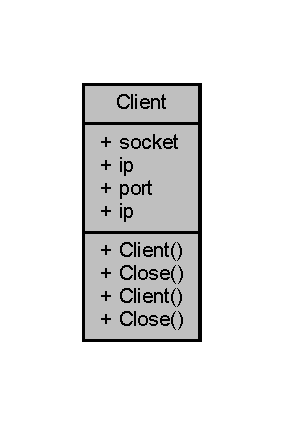
\includegraphics[width=144pt]{struct_client__coll__graph}
\end{center}
\end{figure}
\doxysubsection*{Public Member Functions}
\begin{DoxyCompactItemize}
\item 
\mbox{\Hypertarget{struct_client_a132974d9849fc9318782f74ac6d67ecd}\label{struct_client_a132974d9849fc9318782f74ac6d67ecd}} 
{\bfseries Client} (S\+O\+C\+K\+ET \+\_\+socket, const string \&\+\_\+ip, int \+\_\+port)
\item 
\mbox{\Hypertarget{struct_client_aaf6a8239f1f36ef898d289860d7dacb3}\label{struct_client_aaf6a8239f1f36ef898d289860d7dacb3}} 
void {\bfseries Close} ()
\end{DoxyCompactItemize}
\doxysubsection*{Public Attributes}
\begin{DoxyCompactItemize}
\item 
\mbox{\Hypertarget{struct_client_aab1eb9aade8a3ebb53555a1934f71936}\label{struct_client_aab1eb9aade8a3ebb53555a1934f71936}} 
S\+O\+C\+K\+ET {\bfseries socket}
\item 
\mbox{\Hypertarget{struct_client_a5eaf1ed83e42eec32c685efc35c93e24}\label{struct_client_a5eaf1ed83e42eec32c685efc35c93e24}} 
string {\bfseries ip}
\item 
\mbox{\Hypertarget{struct_client_aad8864d1362eae7c50e53c0d131b7442}\label{struct_client_aad8864d1362eae7c50e53c0d131b7442}} 
int {\bfseries port}
\end{DoxyCompactItemize}


The documentation for this struct was generated from the following file\+:\begin{DoxyCompactItemize}
\item 
src/Server\+Parking.\+cpp\end{DoxyCompactItemize}

\hypertarget{class_parking}{}\section{Parking Class Reference}
\label{class_parking}\index{Parking@{Parking}}


Collaboration diagram for Parking\+:
\nopagebreak
\begin{figure}[H]
\begin{center}
\leavevmode
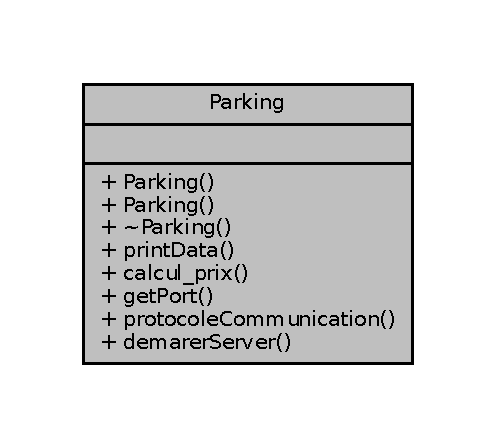
\includegraphics[width=238pt]{class_parking__coll__graph}
\end{center}
\end{figure}
\subsection*{Public Member Functions}
\begin{DoxyCompactItemize}
\item 
\mbox{\hyperlink{class_parking_a71be192e206305ba76ef2c96cd5bbe5a}{Parking}} (int id, float default\+Price, int capacite\+\_\+max, string chemin\+Fichier)
\begin{DoxyCompactList}\small\item\em Construct a new \mbox{\hyperlink{class_parking}{Parking}}\+:\+: \mbox{\hyperlink{class_parking}{Parking}} object. \end{DoxyCompactList}\item 
\mbox{\hyperlink{class_parking_a300004ddbc70c562488cf3f933d5cfb3}{Parking}} (int id, string chemin\+Fichier)
\begin{DoxyCompactList}\small\item\em Construct a new \mbox{\hyperlink{class_parking}{Parking}}\+:\+: \mbox{\hyperlink{class_parking}{Parking}} object. \end{DoxyCompactList}\item 
\mbox{\Hypertarget{class_parking_aba04e48c6e34ae0c1eaee8f3d670e8fb}\label{class_parking_aba04e48c6e34ae0c1eaee8f3d670e8fb}} 
\mbox{\hyperlink{class_parking_aba04e48c6e34ae0c1eaee8f3d670e8fb}{$\sim$\+Parking}} ()
\begin{DoxyCompactList}\small\item\em Destroy the \mbox{\hyperlink{class_parking}{Parking}}\+:\+: \mbox{\hyperlink{class_parking}{Parking}} object. \end{DoxyCompactList}\item 
\mbox{\Hypertarget{class_parking_acddc5b3da5d2769385affe3aad116cb3}\label{class_parking_acddc5b3da5d2769385affe3aad116cb3}} 
void {\bfseries print\+Data} ()
\item 
float \mbox{\hyperlink{class_parking_a41df7b6f534723a56c36f7c06d336f1b}{calcul\+\_\+prix}} (string tab\mbox{[}$\,$\mbox{]})
\item 
\mbox{\Hypertarget{class_parking_a95abbf61891ce84164c19e642756b25b}\label{class_parking_a95abbf61891ce84164c19e642756b25b}} 
int {\bfseries get\+Port} ()
\item 
string \mbox{\hyperlink{class_parking_a4b02969c773d1f1cbe8b895608124a49}{protocole\+Communication}} (string message)
\item 
bool \mbox{\hyperlink{class_parking_a28bcb84c5a6f26d13646253fd69471dd}{demarer\+Server}} ()
\end{DoxyCompactItemize}


\subsection{Constructor \& Destructor Documentation}
\mbox{\Hypertarget{class_parking_a71be192e206305ba76ef2c96cd5bbe5a}\label{class_parking_a71be192e206305ba76ef2c96cd5bbe5a}} 
\index{Parking@{Parking}!Parking@{Parking}}
\index{Parking@{Parking}!Parking@{Parking}}
\subsubsection{\texorpdfstring{Parking()}{Parking()}\hspace{0.1cm}{\footnotesize\ttfamily [1/2]}}
{\footnotesize\ttfamily Parking\+::\+Parking (\begin{DoxyParamCaption}\item[{int}]{id,  }\item[{float}]{default\+Price,  }\item[{int}]{capacite\+\_\+max,  }\item[{string}]{chemin\+Fichier }\end{DoxyParamCaption})}



Construct a new \mbox{\hyperlink{class_parking}{Parking}}\+:\+: \mbox{\hyperlink{class_parking}{Parking}} object. 


\begin{DoxyParams}{Parameters}
{\em id} & \\
\hline
{\em default\+Price} & \\
\hline
{\em capacite\+\_\+max} & \\
\hline
{\em chemin\+Fichier} & \\
\hline
\end{DoxyParams}
\mbox{\Hypertarget{class_parking_a300004ddbc70c562488cf3f933d5cfb3}\label{class_parking_a300004ddbc70c562488cf3f933d5cfb3}} 
\index{Parking@{Parking}!Parking@{Parking}}
\index{Parking@{Parking}!Parking@{Parking}}
\subsubsection{\texorpdfstring{Parking()}{Parking()}\hspace{0.1cm}{\footnotesize\ttfamily [2/2]}}
{\footnotesize\ttfamily Parking\+::\+Parking (\begin{DoxyParamCaption}\item[{int}]{id,  }\item[{string}]{chemin\+Fichier }\end{DoxyParamCaption})}



Construct a new \mbox{\hyperlink{class_parking}{Parking}}\+:\+: \mbox{\hyperlink{class_parking}{Parking}} object. 


\begin{DoxyParams}{Parameters}
{\em id} & \\
\hline
{\em chemin\+Fichier} & \\
\hline
\end{DoxyParams}
Here is the call graph for this function\+:
\nopagebreak
\begin{figure}[H]
\begin{center}
\leavevmode
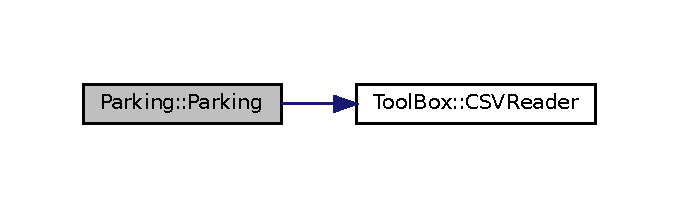
\includegraphics[width=326pt]{class_parking_a300004ddbc70c562488cf3f933d5cfb3_cgraph}
\end{center}
\end{figure}


\subsection{Member Function Documentation}
\mbox{\Hypertarget{class_parking_a41df7b6f534723a56c36f7c06d336f1b}\label{class_parking_a41df7b6f534723a56c36f7c06d336f1b}} 
\index{Parking@{Parking}!calcul\+\_\+prix@{calcul\+\_\+prix}}
\index{calcul\+\_\+prix@{calcul\+\_\+prix}!Parking@{Parking}}
\subsubsection{\texorpdfstring{calcul\+\_\+prix()}{calcul\_prix()}}
{\footnotesize\ttfamily float Parking\+::calcul\+\_\+prix (\begin{DoxyParamCaption}\item[{string}]{tab\mbox{[}$\,$\mbox{]} }\end{DoxyParamCaption})}


\begin{DoxyParams}{Parameters}
{\em tab} & \\
\hline
\end{DoxyParams}
\begin{DoxyReturn}{Returns}
float 
\end{DoxyReturn}
\mbox{\Hypertarget{class_parking_a28bcb84c5a6f26d13646253fd69471dd}\label{class_parking_a28bcb84c5a6f26d13646253fd69471dd}} 
\index{Parking@{Parking}!demarer\+Server@{demarer\+Server}}
\index{demarer\+Server@{demarer\+Server}!Parking@{Parking}}
\subsubsection{\texorpdfstring{demarer\+Server()}{demarerServer()}}
{\footnotesize\ttfamily bool Parking\+::demarer\+Server (\begin{DoxyParamCaption}{ }\end{DoxyParamCaption})}

\begin{DoxyReturn}{Returns}
true 

false 
\end{DoxyReturn}
\mbox{\Hypertarget{class_parking_a4b02969c773d1f1cbe8b895608124a49}\label{class_parking_a4b02969c773d1f1cbe8b895608124a49}} 
\index{Parking@{Parking}!protocole\+Communication@{protocole\+Communication}}
\index{protocole\+Communication@{protocole\+Communication}!Parking@{Parking}}
\subsubsection{\texorpdfstring{protocole\+Communication()}{protocoleCommunication()}}
{\footnotesize\ttfamily string Parking\+::protocole\+Communication (\begin{DoxyParamCaption}\item[{string}]{message }\end{DoxyParamCaption})}


\begin{DoxyParams}{Parameters}
{\em message} & \\
\hline
\end{DoxyParams}
\begin{DoxyReturn}{Returns}
string 
\end{DoxyReturn}


The documentation for this class was generated from the following files\+:\begin{DoxyCompactItemize}
\item 
headers/parking.\+hpp\item 
src/parking.\+cpp\end{DoxyCompactItemize}

\hypertarget{class_t_c_p_socket}{}\doxysection{T\+C\+P\+Socket Class Reference}
\label{class_t_c_p_socket}\index{TCPSocket@{TCPSocket}}


{\ttfamily \#include $<$T\+C\+P\+Socket.\+hpp$>$}



Collaboration diagram for T\+C\+P\+Socket\+:
\nopagebreak
\begin{figure}[H]
\begin{center}
\leavevmode
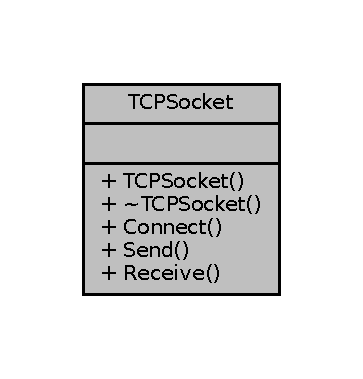
\includegraphics[width=174pt]{class_t_c_p_socket__coll__graph}
\end{center}
\end{figure}
\doxysubsection*{Public Member Functions}
\begin{DoxyCompactItemize}
\item 
\mbox{\hyperlink{class_t_c_p_socket_a7a50427a401d1a6f3209d51818bad901}{T\+C\+P\+Socket}} ()
\begin{DoxyCompactList}\small\item\em Construct a new \mbox{\hyperlink{class_t_c_p_socket_a7a50427a401d1a6f3209d51818bad901}{T\+C\+P\+Socket\+::\+T\+C\+P\+Socket}} object. \end{DoxyCompactList}\item 
\mbox{\hyperlink{class_t_c_p_socket_af357e6923a0f8adbbb8e46fab4523991}{$\sim$\+T\+C\+P\+Socket}} ()
\begin{DoxyCompactList}\small\item\em Destroy the \mbox{\hyperlink{class_t_c_p_socket_a7a50427a401d1a6f3209d51818bad901}{T\+C\+P\+Socket\+::\+T\+C\+P\+Socket}} object. \end{DoxyCompactList}\item 
bool \mbox{\hyperlink{class_t_c_p_socket_ac816c30175550d8d9a14c89c1c5ec8da}{Connect}} (const std\+::string \&ipaddress, unsigned short port)
\begin{DoxyCompactList}\small\item\em Connects an IP Adress to a specific port. \end{DoxyCompactList}\item 
int \mbox{\hyperlink{class_t_c_p_socket_acc5345a54a874aafb3389489f2c1c846}{Send}} (const char $\ast$data, unsigned int len)
\begin{DoxyCompactList}\small\item\em Sends a message trough the socket. \end{DoxyCompactList}\item 
int \mbox{\hyperlink{class_t_c_p_socket_a8341c9364e71e992aa61534dbf88a2a2}{Receive}} (char $\ast$buffer, unsigned int len)
\begin{DoxyCompactList}\small\item\em Recieves a message trough the socket. \end{DoxyCompactList}\end{DoxyCompactItemize}


\doxysubsection{Detailed Description}
S\+A6 -\/ Intelligent Car-\/\+Park 

\doxysubsection{Constructor \& Destructor Documentation}
\mbox{\Hypertarget{class_t_c_p_socket_a7a50427a401d1a6f3209d51818bad901}\label{class_t_c_p_socket_a7a50427a401d1a6f3209d51818bad901}} 
\index{TCPSocket@{TCPSocket}!TCPSocket@{TCPSocket}}
\index{TCPSocket@{TCPSocket}!TCPSocket@{TCPSocket}}
\doxysubsubsection{\texorpdfstring{TCPSocket()}{TCPSocket()}}
{\footnotesize\ttfamily T\+C\+P\+Socket\+::\+T\+C\+P\+Socket (\begin{DoxyParamCaption}{ }\end{DoxyParamCaption})}



Construct a new \mbox{\hyperlink{class_t_c_p_socket_a7a50427a401d1a6f3209d51818bad901}{T\+C\+P\+Socket\+::\+T\+C\+P\+Socket}} object. 

S\+A6 -\/ Intelligent Car-\/\+Park \mbox{\Hypertarget{class_t_c_p_socket_af357e6923a0f8adbbb8e46fab4523991}\label{class_t_c_p_socket_af357e6923a0f8adbbb8e46fab4523991}} 
\index{TCPSocket@{TCPSocket}!````~TCPSocket@{$\sim$TCPSocket}}
\index{````~TCPSocket@{$\sim$TCPSocket}!TCPSocket@{TCPSocket}}
\doxysubsubsection{\texorpdfstring{$\sim$TCPSocket()}{~TCPSocket()}}
{\footnotesize\ttfamily T\+C\+P\+Socket\+::$\sim$\+T\+C\+P\+Socket (\begin{DoxyParamCaption}{ }\end{DoxyParamCaption})}



Destroy the \mbox{\hyperlink{class_t_c_p_socket_a7a50427a401d1a6f3209d51818bad901}{T\+C\+P\+Socket\+::\+T\+C\+P\+Socket}} object. 



\doxysubsection{Member Function Documentation}
\mbox{\Hypertarget{class_t_c_p_socket_ac816c30175550d8d9a14c89c1c5ec8da}\label{class_t_c_p_socket_ac816c30175550d8d9a14c89c1c5ec8da}} 
\index{TCPSocket@{TCPSocket}!Connect@{Connect}}
\index{Connect@{Connect}!TCPSocket@{TCPSocket}}
\doxysubsubsection{\texorpdfstring{Connect()}{Connect()}}
{\footnotesize\ttfamily bool T\+C\+P\+Socket\+::\+Connect (\begin{DoxyParamCaption}\item[{const std\+::string \&}]{ipaddress,  }\item[{unsigned short}]{port }\end{DoxyParamCaption})}



Connects an IP Adress to a specific port. 


\begin{DoxyParams}{Parameters}
{\em ipaddress} & \\
\hline
{\em port} & \\
\hline
\end{DoxyParams}
\begin{DoxyReturn}{Returns}
true if the connection was succesfull, false otherwise. 
\end{DoxyReturn}
Here is the caller graph for this function\+:
\nopagebreak
\begin{figure}[H]
\begin{center}
\leavevmode
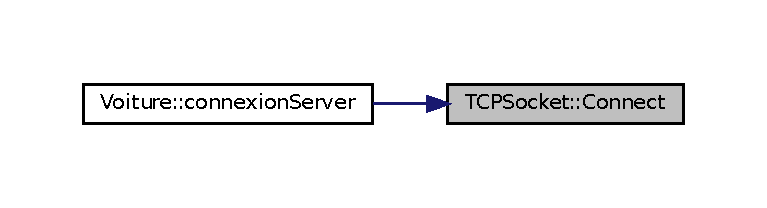
\includegraphics[width=350pt]{class_t_c_p_socket_ac816c30175550d8d9a14c89c1c5ec8da_icgraph}
\end{center}
\end{figure}
\mbox{\Hypertarget{class_t_c_p_socket_a8341c9364e71e992aa61534dbf88a2a2}\label{class_t_c_p_socket_a8341c9364e71e992aa61534dbf88a2a2}} 
\index{TCPSocket@{TCPSocket}!Receive@{Receive}}
\index{Receive@{Receive}!TCPSocket@{TCPSocket}}
\doxysubsubsection{\texorpdfstring{Receive()}{Receive()}}
{\footnotesize\ttfamily int T\+C\+P\+Socket\+::\+Receive (\begin{DoxyParamCaption}\item[{char $\ast$}]{buffer,  }\item[{unsigned int}]{len }\end{DoxyParamCaption})}



Recieves a message trough the socket. 


\begin{DoxyParams}{Parameters}
{\em buffer} & \\
\hline
{\em len} & \\
\hline
\end{DoxyParams}
\begin{DoxyReturn}{Returns}
int 
\end{DoxyReturn}
\mbox{\Hypertarget{class_t_c_p_socket_acc5345a54a874aafb3389489f2c1c846}\label{class_t_c_p_socket_acc5345a54a874aafb3389489f2c1c846}} 
\index{TCPSocket@{TCPSocket}!Send@{Send}}
\index{Send@{Send}!TCPSocket@{TCPSocket}}
\doxysubsubsection{\texorpdfstring{Send()}{Send()}}
{\footnotesize\ttfamily int T\+C\+P\+Socket\+::\+Send (\begin{DoxyParamCaption}\item[{const char $\ast$}]{data,  }\item[{unsigned int}]{len }\end{DoxyParamCaption})}



Sends a message trough the socket. 


\begin{DoxyParams}{Parameters}
{\em data} & \\
\hline
{\em len} & \\
\hline
\end{DoxyParams}
\begin{DoxyReturn}{Returns}
int 
\end{DoxyReturn}


The documentation for this class was generated from the following files\+:\begin{DoxyCompactItemize}
\item 
headers/T\+C\+P\+Socket.\+hpp\item 
src/T\+C\+P\+Socket.\+cpp\end{DoxyCompactItemize}

\hypertarget{class_tool_box}{}\doxysection{Tool\+Box Class Reference}
\label{class_tool_box}\index{ToolBox@{ToolBox}}


Collaboration diagram for Tool\+Box\+:
\nopagebreak
\begin{figure}[H]
\begin{center}
\leavevmode
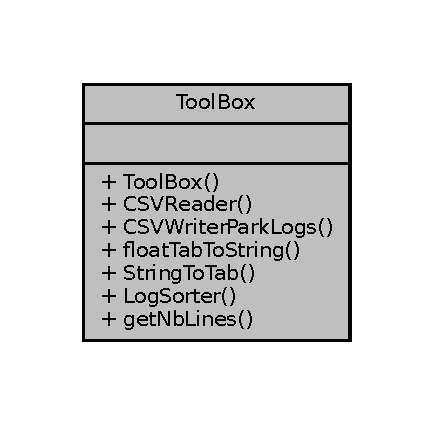
\includegraphics[width=208pt]{class_tool_box__coll__graph}
\end{center}
\end{figure}
\doxysubsection*{Public Member Functions}
\begin{DoxyCompactItemize}
\item 
\mbox{\Hypertarget{class_tool_box_a2dcc60d601f6460bc0c702db398e6279}\label{class_tool_box_a2dcc60d601f6460bc0c702db398e6279}} 
string {\bfseries C\+S\+V\+Reader} (string file, int id)
\item 
bool \mbox{\hyperlink{class_tool_box_a71d8e3e1a4436362c10d1d0df1077893}{C\+S\+V\+Writer\+Park\+Logs}} (string file, string id\+Voiture)
\begin{DoxyCompactList}\small\item\em Write in a C\+SV file at a specific line. Not done yet. \end{DoxyCompactList}\item 
\mbox{\Hypertarget{class_tool_box_a268881f9f0d13d7bf048b7c647376e65}\label{class_tool_box_a268881f9f0d13d7bf048b7c647376e65}} 
string {\bfseries float\+Tab\+To\+String} (vector$<$ float $>$ tab, char delimiter)
\item 
vector$<$ string $>$ \mbox{\hyperlink{class_tool_box_ae43383301f2a0fb0e9b130eff73751d3}{String\+To\+Tab}} (string tab, char delimiter)
\begin{DoxyCompactList}\small\item\em Convert a string to a tab of strings. \end{DoxyCompactList}\item 
\mbox{\Hypertarget{class_tool_box_ae4cf09fc3ad120d68b517e63d02c0f08}\label{class_tool_box_ae4cf09fc3ad120d68b517e63d02c0f08}} 
bool {\bfseries Log\+Sorter} (string file)
\item 
int \mbox{\hyperlink{class_tool_box_a842622e5e6b2cfdf005bfb030837bcf5}{get\+Nb\+Lines}} (string file)
\begin{DoxyCompactList}\small\item\em Sort a C\+SV file by ID. \end{DoxyCompactList}\end{DoxyCompactItemize}


\doxysubsection{Member Function Documentation}
\mbox{\Hypertarget{class_tool_box_a71d8e3e1a4436362c10d1d0df1077893}\label{class_tool_box_a71d8e3e1a4436362c10d1d0df1077893}} 
\index{ToolBox@{ToolBox}!CSVWriterParkLogs@{CSVWriterParkLogs}}
\index{CSVWriterParkLogs@{CSVWriterParkLogs}!ToolBox@{ToolBox}}
\doxysubsubsection{\texorpdfstring{CSVWriterParkLogs()}{CSVWriterParkLogs()}}
{\footnotesize\ttfamily bool Tool\+Box\+::\+C\+S\+V\+Writer\+Park\+Logs (\begin{DoxyParamCaption}\item[{string}]{file,  }\item[{string}]{id\+Voiture }\end{DoxyParamCaption})}



Write in a C\+SV file at a specific line. Not done yet. 


\begin{DoxyParams}{Parameters}
{\em file} & the name of the C\+SV file. \\
\hline
{\em id} & the line number containing the sought information. \\
\hline
\end{DoxyParams}

\begin{DoxyExceptions}{Exceptions}
{\em std\+::runtime\+\_\+error} & Thrown if {\ttfamily file} could not be opened. \\
\hline
\end{DoxyExceptions}
\begin{DoxyReturn}{Returns}
true, false if nothing was written in the file. 
\end{DoxyReturn}
\mbox{\Hypertarget{class_tool_box_a842622e5e6b2cfdf005bfb030837bcf5}\label{class_tool_box_a842622e5e6b2cfdf005bfb030837bcf5}} 
\index{ToolBox@{ToolBox}!getNbLines@{getNbLines}}
\index{getNbLines@{getNbLines}!ToolBox@{ToolBox}}
\doxysubsubsection{\texorpdfstring{getNbLines()}{getNbLines()}}
{\footnotesize\ttfamily int Tool\+Box\+::get\+Nb\+Lines (\begin{DoxyParamCaption}\item[{string}]{file }\end{DoxyParamCaption})}



Sort a C\+SV file by ID. 


\begin{DoxyParams}{Parameters}
{\em file} & the C\+SV file \\
\hline
{\em pos\+Id} & the position of the ID \\
\hline
\end{DoxyParams}

\begin{DoxyExceptions}{Exceptions}
{\em std\+::runtime\+\_\+error} & Thrown if {\ttfamily file} could not be opened. \\
\hline
\end{DoxyExceptions}
\begin{DoxyReturn}{Returns}
true if the operation was successful 

false if the operation wasn\textquotesingle{}t successful
\end{DoxyReturn}
Counts the number of line of a file


\begin{DoxyParams}{Parameters}
{\em file} & \\
\hline
\end{DoxyParams}
\begin{DoxyReturn}{Returns}
int 
\end{DoxyReturn}
\mbox{\Hypertarget{class_tool_box_ae43383301f2a0fb0e9b130eff73751d3}\label{class_tool_box_ae43383301f2a0fb0e9b130eff73751d3}} 
\index{ToolBox@{ToolBox}!StringToTab@{StringToTab}}
\index{StringToTab@{StringToTab}!ToolBox@{ToolBox}}
\doxysubsubsection{\texorpdfstring{StringToTab()}{StringToTab()}}
{\footnotesize\ttfamily vector$<$ string $>$ Tool\+Box\+::\+String\+To\+Tab (\begin{DoxyParamCaption}\item[{string}]{msg,  }\item[{char}]{delimiter }\end{DoxyParamCaption})}



Convert a string to a tab of strings. 


\begin{DoxyParams}{Parameters}
{\em msg} & the string \\
\hline
{\em delimiter} & the delimiter \\
\hline
\end{DoxyParams}
\begin{DoxyReturn}{Returns}
vector$<$string$>$ 
\end{DoxyReturn}
Here is the caller graph for this function\+:
\nopagebreak
\begin{figure}[H]
\begin{center}
\leavevmode
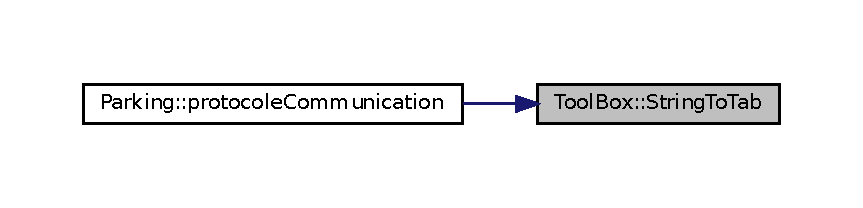
\includegraphics[width=350pt]{class_tool_box_ae43383301f2a0fb0e9b130eff73751d3_icgraph}
\end{center}
\end{figure}


The documentation for this class was generated from the following files\+:\begin{DoxyCompactItemize}
\item 
doc/uml.\+txt\item 
headers/Tool\+Box.\+hpp\item 
src/Tool\+Box.\+cpp\end{DoxyCompactItemize}

\hypertarget{class_voiture}{}\section{Voiture Class Reference}
\label{class_voiture}\index{Voiture@{Voiture}}


Collaboration diagram for Voiture\+:
\nopagebreak
\begin{figure}[H]
\begin{center}
\leavevmode
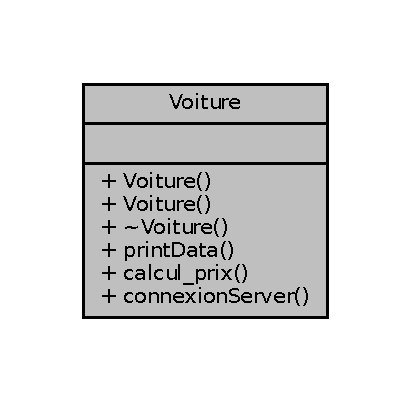
\includegraphics[width=197pt]{class_voiture__coll__graph}
\end{center}
\end{figure}
\subsection*{Public Member Functions}
\begin{DoxyCompactItemize}
\item 
\mbox{\hyperlink{class_voiture_a9f8646dde1dd92d80cf56b975bba97c2}{Voiture}} (int id, string file\+Path)
\begin{DoxyCompactList}\small\item\em \mbox{\hyperlink{class_voiture}{Voiture}} Constructor, extracts information from a C\+SV file. \end{DoxyCompactList}\item 
\mbox{\hyperlink{class_voiture_a77002698169f77149f6bd92f875b86cf}{Voiture}} (int id, string name, string marque, string statut, string handicap, string age, string heure)
\begin{DoxyCompactList}\small\item\em \mbox{\hyperlink{class_voiture}{Voiture}} Constructor. \end{DoxyCompactList}\item 
\mbox{\Hypertarget{class_voiture_afe85820a993b6908d0fdb524245e5133}\label{class_voiture_afe85820a993b6908d0fdb524245e5133}} 
\mbox{\hyperlink{class_voiture_afe85820a993b6908d0fdb524245e5133}{$\sim$\+Voiture}} ()
\begin{DoxyCompactList}\small\item\em \mbox{\hyperlink{class_voiture}{Voiture}} Destructor. \end{DoxyCompactList}\item 
\mbox{\Hypertarget{class_voiture_a3d786c35df10757794b241134f5e2f2e}\label{class_voiture_a3d786c35df10757794b241134f5e2f2e}} 
void \mbox{\hyperlink{class_voiture_a3d786c35df10757794b241134f5e2f2e}{print\+Data}} ()
\begin{DoxyCompactList}\small\item\em Prints the car informations. \end{DoxyCompactList}\item 
float \mbox{\hyperlink{class_voiture_a1cd531495d64c694292374d96724c654}{calcul\+\_\+prix}} ()
\begin{DoxyCompactList}\small\item\em Method that calculates the park price the car owner wants to pay. \end{DoxyCompactList}\item 
bool \mbox{\hyperlink{class_voiture_abbc7a9f5a9e05a92b75623ff87bee85c}{connexion\+Server}} (int port)
\begin{DoxyCompactList}\small\item\em Method used to connect the car with a specific \mbox{\hyperlink{class_parking}{Parking}} using sockets. \end{DoxyCompactList}\end{DoxyCompactItemize}


\subsection{Constructor \& Destructor Documentation}
\mbox{\Hypertarget{class_voiture_a9f8646dde1dd92d80cf56b975bba97c2}\label{class_voiture_a9f8646dde1dd92d80cf56b975bba97c2}} 
\index{Voiture@{Voiture}!Voiture@{Voiture}}
\index{Voiture@{Voiture}!Voiture@{Voiture}}
\subsubsection{\texorpdfstring{Voiture()}{Voiture()}\hspace{0.1cm}{\footnotesize\ttfamily [1/2]}}
{\footnotesize\ttfamily Voiture\+::\+Voiture (\begin{DoxyParamCaption}\item[{int}]{id,  }\item[{string}]{file\+Path }\end{DoxyParamCaption})}



\mbox{\hyperlink{class_voiture}{Voiture}} Constructor, extracts information from a C\+SV file. 


\begin{DoxyParams}{Parameters}
{\em id} & the id number of the car. \\
\hline
{\em file\+Path} & path of the C\+SV file. \\
\hline
\end{DoxyParams}
\begin{DoxyReturn}{Returns}
the object \mbox{\hyperlink{class_voiture}{Voiture}}. 
\end{DoxyReturn}
Here is the call graph for this function\+:
\nopagebreak
\begin{figure}[H]
\begin{center}
\leavevmode
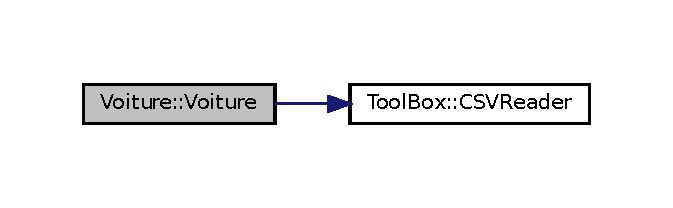
\includegraphics[width=323pt]{class_voiture_a9f8646dde1dd92d80cf56b975bba97c2_cgraph}
\end{center}
\end{figure}
\mbox{\Hypertarget{class_voiture_a77002698169f77149f6bd92f875b86cf}\label{class_voiture_a77002698169f77149f6bd92f875b86cf}} 
\index{Voiture@{Voiture}!Voiture@{Voiture}}
\index{Voiture@{Voiture}!Voiture@{Voiture}}
\subsubsection{\texorpdfstring{Voiture()}{Voiture()}\hspace{0.1cm}{\footnotesize\ttfamily [2/2]}}
{\footnotesize\ttfamily Voiture\+::\+Voiture (\begin{DoxyParamCaption}\item[{int}]{id,  }\item[{string}]{name,  }\item[{string}]{marque,  }\item[{string}]{statut,  }\item[{string}]{handicap,  }\item[{string}]{age,  }\item[{string}]{heure }\end{DoxyParamCaption})}



\mbox{\hyperlink{class_voiture}{Voiture}} Constructor. 


\begin{DoxyParams}{Parameters}
{\em id} & the id number of the car. \\
\hline
{\em name} & the name of the car. \\
\hline
{\em marque} & the brand of the car. \\
\hline
{\em statut} & the car owner\textquotesingle{}s status. \\
\hline
{\em handicap} & if the owner has a handicap. \\
\hline
{\em age} & the age of the car owner. \\
\hline
{\em heure} & the number of hour the owner is willing to park. \\
\hline
\end{DoxyParams}
\begin{DoxyReturn}{Returns}
the object \mbox{\hyperlink{class_voiture}{Voiture}}. 
\end{DoxyReturn}


\subsection{Member Function Documentation}
\mbox{\Hypertarget{class_voiture_a1cd531495d64c694292374d96724c654}\label{class_voiture_a1cd531495d64c694292374d96724c654}} 
\index{Voiture@{Voiture}!calcul\+\_\+prix@{calcul\+\_\+prix}}
\index{calcul\+\_\+prix@{calcul\+\_\+prix}!Voiture@{Voiture}}
\subsubsection{\texorpdfstring{calcul\+\_\+prix()}{calcul\_prix()}}
{\footnotesize\ttfamily float Voiture\+::calcul\+\_\+prix (\begin{DoxyParamCaption}{ }\end{DoxyParamCaption})}



Method that calculates the park price the car owner wants to pay. 

This method uses different data such as the owner status, if he has a handicap, his age and the time he wants to stay.

\begin{DoxyReturn}{Returns}
prix, the fiual price. 
\end{DoxyReturn}
\mbox{\Hypertarget{class_voiture_abbc7a9f5a9e05a92b75623ff87bee85c}\label{class_voiture_abbc7a9f5a9e05a92b75623ff87bee85c}} 
\index{Voiture@{Voiture}!connexion\+Server@{connexion\+Server}}
\index{connexion\+Server@{connexion\+Server}!Voiture@{Voiture}}
\subsubsection{\texorpdfstring{connexion\+Server()}{connexionServer()}}
{\footnotesize\ttfamily bool Voiture\+::connexion\+Server (\begin{DoxyParamCaption}\item[{int}]{port }\end{DoxyParamCaption})}



Method used to connect the car with a specific \mbox{\hyperlink{class_parking}{Parking}} using sockets. 


\begin{DoxyParams}{Parameters}
{\em port} & the port of the \mbox{\hyperlink{class_parking}{Parking}}\textquotesingle{}s server. \\
\hline
\end{DoxyParams}
\begin{DoxyReturn}{Returns}
false if the \mbox{\hyperlink{class_voiture}{Voiture}} can\textquotesingle{}t connect, true otherwise. 
\end{DoxyReturn}
Here is the call graph for this function\+:
\nopagebreak
\begin{figure}[H]
\begin{center}
\leavevmode
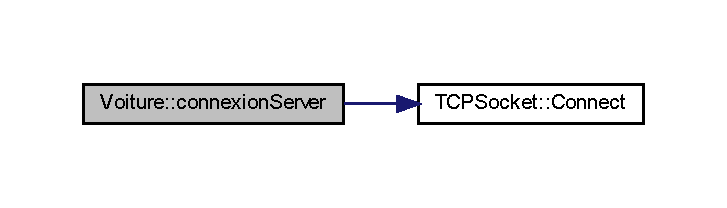
\includegraphics[width=350pt]{class_voiture_abbc7a9f5a9e05a92b75623ff87bee85c_cgraph}
\end{center}
\end{figure}


The documentation for this class was generated from the following files\+:\begin{DoxyCompactItemize}
\item 
headers/voiture.\+hpp\item 
src/voiture.\+cpp\end{DoxyCompactItemize}

%--- End generated contents ---

% Index
\backmatter
\newpage
\phantomsection
\clearemptydoublepage
\addcontentsline{toc}{chapter}{Index}
\printindex

\end{document}
